\chapter{The K--Ar system}
\label{sec:K-Ar}

Potassium has three naturally occurring isotopes: $^{39}$K, $^{40}$K
and $^{41}$K. $^{40}$K is radioactive and undergoes branched decay to
$^{40}$Ca (by electron emission $\lambda_{\beta-} = 4.962 \times
10^{-10} yr^{-1}$) and $^{40}$Ar (by electron capture $\lambda_{e} =
0.581 \times 10^{-10} yr^{-1}$) with a combined half life of 1.248
billion years. The positron emission mechanism mentioned in Chapter
\ref{sec:radioactivity} has an extremely long half life and can
therefore safely be neglected. In addition to $^{40}$Ar, argon has two
more stable isotopes: $^{36}$Ar and $^{38}$Ar. Argon makes up
$\sim$1\% of the terrestrial atmosphere, with a fixed isotopic
composition of $^{40}$Ar/$^{36}$Ar = 298.5 and $^{38}$Ar/$^{36}$Ar =
0.187. The argon contained in K-bearing minerals is made up of a
mixture of radiogenic ($^{40}$Ar$^*$) and non-radiogenic gas
($^{40}$Ar$_\circ$):

\begin{equation}
\begin{array}{rl}
^{40}Ar & = {}^{40}Ar_\circ + {}^{40}Ar^*\\ 
\mbox{where~} {}^{40}Ar^* & =
  \frac{\lambda_e}{\lambda} {}^{40}K \left( e^{\lambda t} - 1 \right)
\end{array}
\label{eq:Ar}
\end{equation}

with $\lambda$ the total decay constant of $^{40}$K ($\lambda =
\lambda_e + \lambda_{\beta-}$ = $5.543 \times 10^{-10} yr^{-1}$).

\section{K-Ar dating}

The $^{40}$K $\rightarrow$ $^{40}$Ar$^*$ decay scheme forms the basis
of the K-Ar geochronometer, with the following age equation:

\begin{equation}
t = \frac{1}{\lambda} \ln\left[ 1 + \frac{\lambda}{\lambda_e}
  \left(\frac{^{40}Ar^*}{^{40}K}\right) \right]
\label{eq:K-Ar}
\end{equation}

Taking into account the `contaminated' (aka `excess' or `inherited')
argon component $^{40}Ar_\circ$ and analysing several cogenetic rocks
or minerals with different K (and therefore $^{40}Ar^*$) contents, an
\emph{isochron} equation can be formed by division through $^{36}$Ar:

\begin{equation}
\frac{^{40}Ar}{^{36}Ar} = \left(\frac{^{40}Ar}{^{36}Ar}\right)_\circ +
\frac{\lambda_e}{\lambda} \frac{^{40}K}{^{36}Ar} \left( e^{\lambda t} - 1 \right)
\label{eq:K-Ar-isochron}
\end{equation}

which can be solved for t. Alternatively, we can simply assume that
all the inherited argon has an atmospheric origin, so that
$({}^{40}Ar/{}^{36}Ar)_\circ = 298.5$.

\section{$^{40}$Ar/$^{39}$Ar dating}
\label{sec:Ar-Ar}

From an analytical perspective, K-Ar dating is a two step
process. Because K (an alkali metal) and Ar (a noble gas) cannot be
measured on the same analytical equipment, they must be analysed
separately on two different aliquots of the same sample.  This
limitation is overcome by the $^{40}$Ar/$^{39}$Ar technique, which is
a clever variation of the K-Ar method. The idea is to subject the
sample to neutron irradiation and convert a small fraction of the
$^{39}$K to synthetic $^{39}$Ar, which has a half life of 269
years. The age equation can then be rewritten as follows:

\begin{equation}
t_x = \frac{1}{\lambda} \ln\left[
1 + J \left(\frac{^{40}Ar^*}{^{39}Ar}\right)_x 
\right]
\label{eq:Ar-Ar}
\end{equation}

where `x' stands for `sample' and J is a constant of proportionality
which encapsulates the efficiency of the $^{39}$K (n,p) $^{39}$Ar
reaction and into which the factor $\lambda/\lambda_e$ is folded as
well.  The J-value can be determined by analysing a standard of known
age t$_s$ which was co-irradiated with the sample:

\begin{equation}
t_s = \frac{1}{\lambda} \ln\left[
1 + J \left(\frac{^{40}Ar^*}{^{39}Ar}\right)_s 
\right]
\label{eq:J}
\end{equation}

In which the subscript `s' stands for `standard'. The great advantage
of equation \ref{eq:Ar-Ar} over \ref{eq:K-Ar} is that all measurements
can be completed on the same aliquot and using a single instrument,
namely a noble gas mass spectrometer, which can analyse extremely
small (down to $\mu$g-sized) samples.\\

The $^{40}$Ar/$^{39}$Ar-method also allows the analyst to investigate
the extent of \emph{argon loss} by means of stepwise heating
experiments.  This is done by degassing the sample under ultra-high
vacuum conditions in a resistance furnace. At low temperatures, the
weakly bound Ar is released, whereas the strongly bound Ar is released
from the crystal lattice at high temperatures until the sample
eventually melts. Plotting the \emph{apparent ages} against the
cumulative fraction of $^{39}$Ar released yields an
$^{40}$Ar/$^{39}$Ar age spectrum (Figure \ref{fig:Ar-Ar}).  If a rock
or mineral has remained closed since its formation, the
$^{40}$Ar/$^{39}$Ar-ratio should remain constant over the course of
the different heating steps, forming an `age plateau'. More complex
(e.g. rising) release spectra, on the other hand, are diagnostic of
complex thermal histories featuring partial argon loss. `saddle'
shaped release spectra are indicative of `excess' argon. The
composition of the inherited argon gas can be determined using a
variant of the isochron method, assuming that all ${}^{36}Ar$ is
inherited:

\begin{equation}
\frac{{}^{40}Ar}{{}^{36}Ar} =
\left(\frac{{}^{40}Ar}{{}^{36}Ar}\right)_\circ +
\frac{{}^{39}Ar}{{}^{36}Ar}\frac{e^{\lambda t} - 1}{J}
\label{eq:Ar-Ar-isochron}
\end{equation}

If the Ar contamination is constant throughout the entire sample, then
the $\frac{^{40}Ar}{^{36}Ar}$-measurements will be arranged along a
linear trend whose slope is a function of $\frac{^{40}Ar^*}{^{39}Ar}$
and, hence, the age.\\

\ifpdf
\ifuclnotes
\begin{figure}[!ht]
  \centering
  \def\svgwidth{.7\textwidth}
  \input{Ar-Ar.pdf_tex}
  \caption{$^{40}$Ar/$^{39}$Ar age spectra obtained by stepwise
    heating of three different K-bearing minerals. Biotite exhibits a
    flat `plateau', indicating a simple history of rapid
    crystallisation and/or cooling. K-feldspar shows a rising age
    spectrum, consistent with a more complex evolution comprising
    multiple growth phases and/or thermal resetting. Finally,
    hornblende shows a `U-shaped' release spectrum in which the first
    heating step releases a large amount of `excess' argon
    \citep[modified from][]{allegre2008}.}
  \label{fig:Ar-Ar}
\end{figure}
\else % end of uclnotes
\begin{figure}[!ht]
\noindent\begin{minipage}[t]{.55\textwidth}
\strut\vspace*{-\baselineskip}\newline
\def\svgwidth{\textwidth}
\input{Ar-Ar.pdf_tex}
\end{minipage}
\begin{minipage}[t]{.45\textwidth}
  \captionof{figure}{$^{40}$Ar/$^{39}$Ar age spectra obtained by stepwise
    heating of three different K-bearing minerals. Biotite exhibits a
    flat `plateau', indicating a simple history of rapid
    crystallisation and/or cooling. K-feldspar shows a rising age
    spectrum, consistent with a more complex evolution comprising
    multiple growth phases and/or thermal resetting. Finally,
    hornblende shows a `U-shaped' release spectrum in which the first
    heating step releases a large amount of `excess' argon
    \citep[modified from][]{allegre2008}.}
  \label{fig:Ar-Ar}
\end{minipage}
\end{figure}
\fi % end of pdf
\else
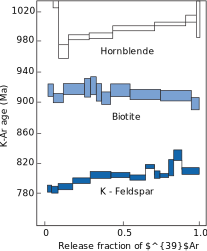
\includegraphics[width=10cm]{../figures/Ar-Ar.png}
  \captionof{figure}{$^{40}$Ar/$^{39}$Ar age spectra obtained by stepwise
    heating of three different K-bearing minerals. Biotite exhibits a
    flat `plateau', indicating a simple history of rapid
    crystallisation and/or cooling. K-feldspar shows a rising age
    spectrum, consistent with a more complex evolution comprising
    multiple growth phases and/or thermal resetting. Finally,
    hornblende shows a `U-shaped' release spectrum in which the first
    heating step releases a large amount of `excess' argon
    \citep[modified from][]{allegre2008}.}
  \label{fig:Ar-Ar}
\fi

\section{Applications}
\label{sec:Ar-applications}

The K-Ar and $^{40}$Ar/$^{39}$Ar-methods are some of the most widely
used geochronometers and important tools in the calibration of the
geologic time scale. The method is applicable to rocks and minerals
$>$ 10$^6$yr. Obviously, younger materials require more careful
treatment of the inherited argon components.

\begin{itemize}
\item{Magmatic rocks:} formation ages can only be obtained for rapidly
  cooled volcanic rocks, using either mineral separates (sanidine,
  biotite, hornblende) or whole rocks. Pyroclastics and obsidian may
  yield reliable ages only if they are unaltered and contain little
  non-radiogenic argon. Plutonic rocks typically cool much slower than
  volcanic rocks and generally yield cooling ages rather than
  formation ages.
\item{Sedimentary rocks:} K-Ar dating of \emph{authigenic} mineral
  phases has often been attempted but remains difficult. Glauconite
  has been used successfully in some cases. Dating detrital minerals
  such as white mica (muscovite, phengite) in fluvial sediments is
  frequently used to study the metamorphic history of the hinterland.
\item{Metamorphic rocks:} pelitic metamorphic rocks tend to be rich in
  K-bearing micas and amphiboles, which can easily be dated with the
  K-Ar and $^{40}$Ar/$^{39}$Ar methods, but require careful
  interpretation. In high grade metamorphic terranes, the apparent
  ages can either reflect the metamorphic crystallisation history or
  the postmetamorphic cooling history. Low grade metamorphic terranes,
  on the other hand, carry a risk of containing inherited argon
  components from previous evolutionary stages.
\end{itemize}
